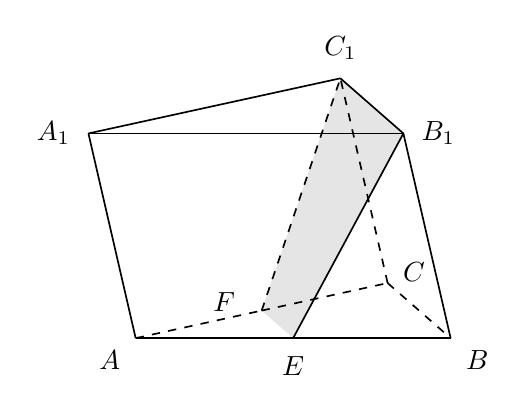
\begin{tikzpicture}[x=1cm,y=1cm,line width=.6pt]
% Triangular prism ABC-A1B1C1, E midpoint of AB, F midpoint of AC.
% Shaded quadrilateral E-B1-C1-F.
\coordinate (A) at (0,0);
\coordinate (E) at (2,0);
\coordinate (B) at (4,0);
\coordinate (F) at (1.6,0.35);
\coordinate (C) at (3.2,0.7);
\coordinate (Aone) at (-0.6,2.6);
\coordinate (Bone) at (3.4,2.6);
\coordinate (Cone) at (2.6,3.3);
% shaded section first (gray block, keeps boundary)
\fill[gray!20] (E) -- (Bone) -- (Cone) -- (F) -- cycle;
% bottom face
\draw (A) -- (E) -- (B);
\draw[dashed] (A) -- (F);
\draw[dashed] (F) -- (C);
\draw[dashed] (C) -- (B);

% lateral + top
\draw (A) -- (Aone);
\draw (B) -- (Bone);
\draw[dashed] (F) -- (Cone);
\draw (E) -- (Bone);
\draw (Aone) -- (Bone);
\draw (Aone) -- (Cone);
\draw (Cone) -- (Bone);
\draw[dashed] (C) -- (Cone);

% labels offset clear of strokes
\node[below left,xshift=-2pt,yshift=-1pt] at (A) {$A$};
\node[below,yshift=-3pt] at (E) {$E$};
\node[below right,xshift=2pt,yshift=-1pt] at (B) {$B$};
\node[left,xshift=-6pt,yshift=3pt] at (F) {$F$};
\node[right,xshift=2pt,yshift=4pt] at (C) {$C$};
\node[left,xshift=-3pt] at (Aone) {$A_{1}$};
\node[right,xshift=3pt] at (Bone) {$B_{1}$};
\node[above,yshift=3pt] at (Cone) {$C_{1}$};
\end{tikzpicture}
